\paragraph{Sơ đồ tuần tự luồng xem trang chủ}

Luồng nghiệp vụ này mô tả
quá trình
Web Frontend
yêu cầu các thông tin cần thiết
từ các dịch vụ thông qua
API Gateway
để hiển thị đầy đủ giao diện trang chủ cho
Khách vãng lai (Guest).

\begin{figure}[H]
\centering
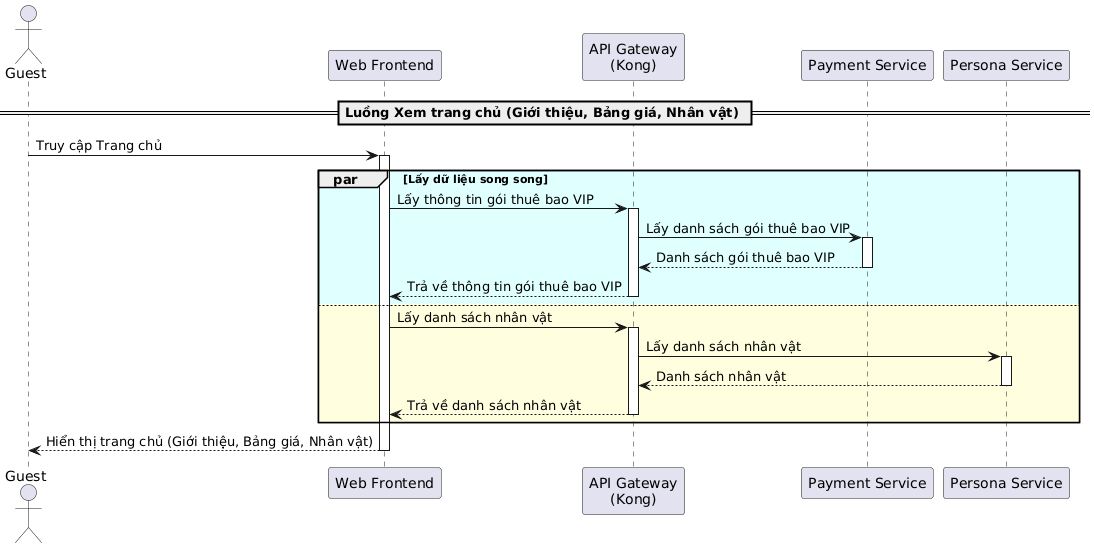
\includegraphics[width=0.95\textwidth]{contents/Sequence/UML-Sequence-GuestHomeOverview.png}
\caption{Sơ đồ tuần tự luồng xem trang chủ}
\end{figure}

\begin{table}[H]
\centering
\renewcommand{\arraystretch}{1.3}

\begin{tabular}{|l|l|p{5cm}|}
\hline
\textbf{Thành phần} & \textbf{Phân loại} & \textbf{Vai trò trong hệ thống} \\ \hline
Guest & Actor & Khách vãng lai truy cập vào hệ thống. \\ \hline
Web Frontend & Component & Giao diện web Next.js. \\ \hline
API Gateway (Kong) & Component & Cổng API chuyển tiếp các yêu cầu API. \\ \hline
Persona Service & Microservice & Cung cấp danh sách các nhân vật và URL tệp giọng nói mẫu. \\ \hline
Payment Service & Microservice & Cung cấp thông tin các gói thuê bao VIP và bảng giá dịch vụ. \\ \hline
\end{tabular}
\caption{Các thành phần tham gia luồng xem trang chủ}
\end{table}

\subparagraph{Mô tả tổng quan}

\begin{itemize}

\item \textbf{Truy cập trang chủ:}
Khách vãng lai truy cập
vào trang chủ của hệ thống.

\item \textbf{Tải bảng giá:}
Giao diện hiển thị
thông tin giới thiệu tĩnh
và gửi yêu cầu lấy bảng giá các gói thuê bao VIP từ dịch vụ thanh toán qua cổng API.

\item \textbf{Tải danh sách nhân vật:}
Giao diện gửi yêu cầu lấy danh sách các nhân vật
kèm tệp âm thanh mẫu từ dịch vụ nhân vật qua cổng API.

\item \textbf{Hiển thị thông tin:}
Giao diện hiển thị bảng giá dịch vụ
và danh sách nhân vật lên màn hình để khách vãng lai tìm hiểu thông tin.
\end{itemize}
